
\documentclass[usenames,dvipsnames]{beamer}
\mode<presentation>{\usetheme{Warsaw}}
\usepackage{textpos} %package for text positioning

%%%%%%%%%%%%%%%%%%%%%%%%%%%%%%%%%%%%%%%%%%%%%%%%%%%%%%%%%%%%%%%%%%%%%%%%%%%%%%%%%%%%
%Normal Math Packages
\usepackage{amsmath}
\usepackage{amsfonts}
\usepackage{enumerate}
\usepackage{amsmath}
\usepackage{mathtools}
\usepackage{tikz-cd}
\usepackage{ragged2e}
\usepackage{mathrsfs}
\usepackage{xcolor}
\usepackage{soul}
%%%%%%%%%%%%%%%%%%%%%%%%%%%%%%%%%%%%%%%%%%%%%%%%%%%%%%%%%%%%%%%%%%%%%%%%%%%%%%%%%%%%

%%%%%%%%%%%%%%%%%%%%%%%%%%%%%%%%%%%%%%%%%%%%%%%%%%%%%%%%%%%%%%%%%%%%%%%%%%%%%%%%%%%%
%Created Commands
\theoremstyle{definition}
\newtheorem*{remark}{Remark}
\newtheorem*{question}{Question}
\newtheorem*{answer}{Answer}
%\newtheorem*{definition}{Definition}
%\newtheorem*{definitions}{Definitions}

\theoremstyle{theorem}
\newtheorem*{proposition}{Proposition}
\newtheorem*{axiom}{Axiom}

\newcommand{\R}{\mathbb{R}}
\newcommand{\Q}{\mathbb{Q}}
\newcommand{\F}{\mathbb{F}}
\newcommand{\A}{\mathcal{A}}
\newcommand{\N}{\mathbb{N}}
\newcommand{\C}{\mathbb{C}}
\newcommand{\opO}{\mathcal{O}}
\newcommand{\states}{\mathcal{S}}
\newcommand{\position}{\boldsymbol{\gamma}}
\newcommand{\velocity}{\boldsymbol{\dot{\gamma}}}
%%%%%%%%%%%%%%%%%%%%%%%%%%%%%%%%%%%%%%%%%%%%%%%%%%%%%%%%%%%%%%%%%%%%%%%%%%%%%%%%%%%%

%%%%%%%%%%%%%%%%%%%%%%%%%%%%%%%%%%%%%%%%%%%%%%%%%%%%%%%%%%%%%%%%%%%%%%%%%%%%%%%%%%%%
%Pseudocode
\usepackage{algorithm}
\usepackage[noend]{algpseudocode}
%%%%%%%%%%%%%%%%%%%%%%%%%%%%%%%%%%%%%%%%%%%%%%%%%%%%%%%%%%%%%%%%%%%%%%%%%%%%%%%%%%%%


%%%%%%%%%%%%%%%%%%%%%%%%%%%%%%%%%%%%%%%%%%%%%%%%%%%%%%%%%%%%%%%%%%%%%%%%%%%%%%%%%%%%
%Remove buttons
\setbeamertemplate{navigation symbols}{}

%Stuff to make things look good
% Color modification
\setbeamercolor{structure}{fg=green!30!black}% to modify  immediately all palettes
\setbeamercolor{title}{fg=white}
\setbeamercolor{title in head/foot}{fg=yellow}

%Size Modification
\setbeamerfont{frametitle}{size=\small}

% position the logo
\addtobeamertemplate{frametitle}{}{%
\begin{textblock*}{1cm}(\textwidth,-1.1cm)

\includegraphics[height=.9cm,width=.9cm,keepaspectratio]{csu.png}
\end{textblock*}}

% Text Positioning
\usepackage[absolute,overlay]{textpos}
%%%%%%%%%%%%%%%%%%%%%%%%%%%%%%%%%%%%%%%%%%%%%%%%%%%%%%%%%%%%%%%%%%%%%%%%%%%%%%%%%%%%

%Font
%\fontfamily{cmr}\selectfont
\usefonttheme{serif}

%Colors and stuf
\usepackage{color, soul, xcolor} % Colored text and highlighting, respectively
\usepackage{tikz-cd} % For commutative diagrams

%% preamble
\title{Harmonic Maps and Gradient Flow}
\subtitle{Math 546 Project}
\author{Colin Roberts}

\begin{document}

%%Title Frame
{
\setbeamertemplate{headline}{}
\addtobeamertemplate{frametitle}{\vspace*{-0.9\baselineskip}}{}
\begin{frame}
\titlepage
\end{frame}
}

%Table of contents slide

%\AtBeginSection[]
%{
%	\begin{frame}{Table of Contents}
%		\tableofcontents[currentsection]
%	\end{frame}
%}

%%%%%%%%%%%%%%%%%%%%%%%%%%%%%%%%%%%%%%%%%%%%%%%%%%%%%%%%%%%%%%%%%%%%%%%%%%%%%%%
%%%%%%%%%%%%%%%%%%%%%%%%%%%%%%%%%%%%%%%%%%%%%%%%%%%%%%%%%%%%%%%%%%%%%%%%%%%%%%%
\section{Overview}
    
    \subsection{Motivation}
        
        \begin{frame}{The Motivating Questions}
            \begin{question}
            What is a physically meaningful energy functional?
            \end{question}
            
            \begin{question}
            What are the functions that minimize this energy?
            \end{question}
            
            \begin{question}
            Is there a method or algorithm to search for an optimizer by starting at any point in our space?
            \end{question}
        \end{frame}
        
    \begin{frame}{Applications}
    \begin{itemize}
    \begin{minipage}{0.45\linewidth}
    \item[] \textbf{\underline{Real World Applications}}
    \item Building 3D (printing) structures.
    \item Machine learning.
    \item Smoothing of data.
\end{minipage}
\begin{minipage}{0.5\linewidth}
    \item[] \textbf{\underline{Mathematics Applications}}
    \item Framework for optimization problems.
    \item Existence of minimal mappings.
    \item Solution to the Poincar\'e conjecture.
\end{minipage}
    \end{itemize}
    \end{frame}

\begin{frame}{The Gyroid}
    \begin{figure}[H]
        \centering
        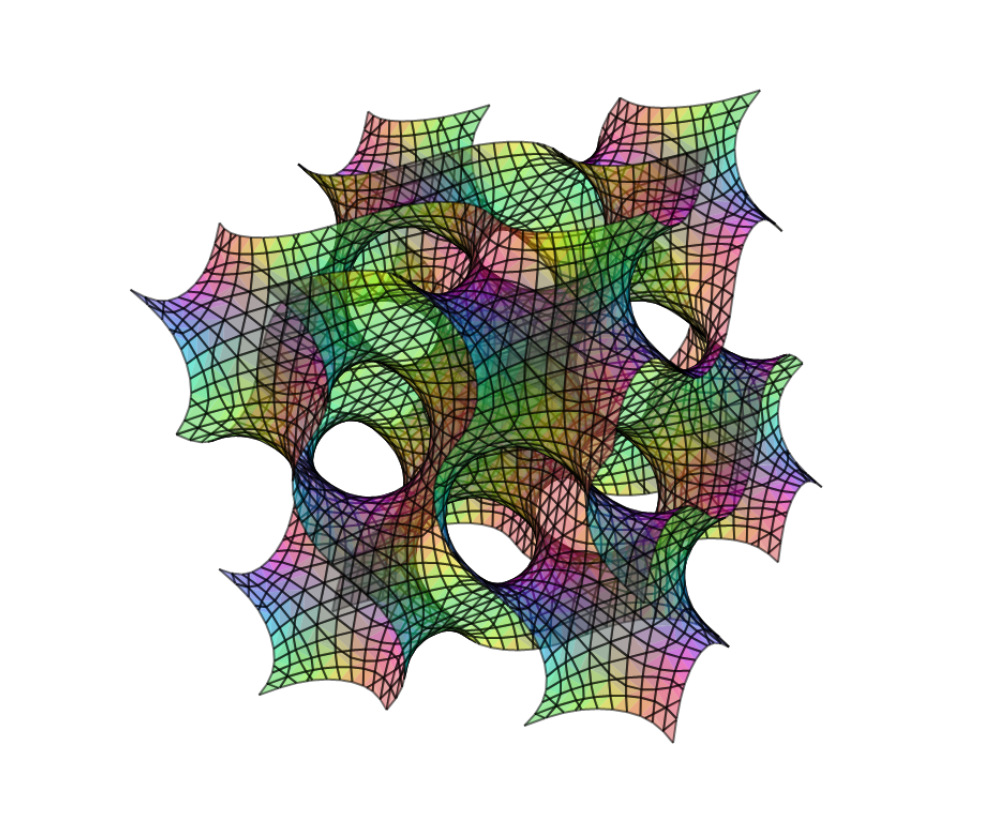
\includegraphics[width=.6\textwidth]{images/gyroid_fixed.png}
    \end{figure}
\end{frame}

\begin{frame}{Applications}
\begin{itemize}
    \item Existence of minimal surfaces follows from existence of solutions to heat equation.
    \item Ricci flow with surgery- Perelmen's solution to the Poincare conjecture
\end{itemize}
\end{frame}
        
        
        %% Is this frame the best?
        % \begin{frame}{Particle Motion}
        % Kinematic motion follows the shortest possible paths.
        % \begin{itemize}
        %     \item (Non-constrained) What is the shortest path a particle can take between two points?
        %     \item (Constrained) What is the shortest path a particle living on a sphere can take between two points?
        % \end{itemize}
        % \vspace*{.25cm}
        % Dynamical motion follows the paths that best utilize available energy (least action principal).
        % \begin{itemize}
        %     \item (Non-constrained) What is the path of a particle in the presence of a gravitational field?
        %     \item (Constrained) What is the path of a particle living on a sphere in the presence of a gravitational field?
        % \end{itemize}
        % \end{frame}
    
        
        \begin{frame}{The Motivating Problems from Geometry and Physics}
        % \begin{textblock*}{6cm}(5cm,-1cm)
        \begin{itemize}
\begin{minipage}{0.55\linewidth}
    \item[] \textbf{\underline{Geometry}}
    \item Geodesics
    \item Minimal Submanifolds
    \item Gradient Flow
\end{minipage}
\begin{minipage}{0.4\linewidth}
    \item[] \textbf{\underline{Physics}}
    \item Free Particles
    \item Elastic Materials
    \item Heat Flow
\end{minipage}
\end{itemize}
            
            % \end{textblock*}
            % \begin{textblock*}{5cm}(-.5cm,-1.75cm)
            % 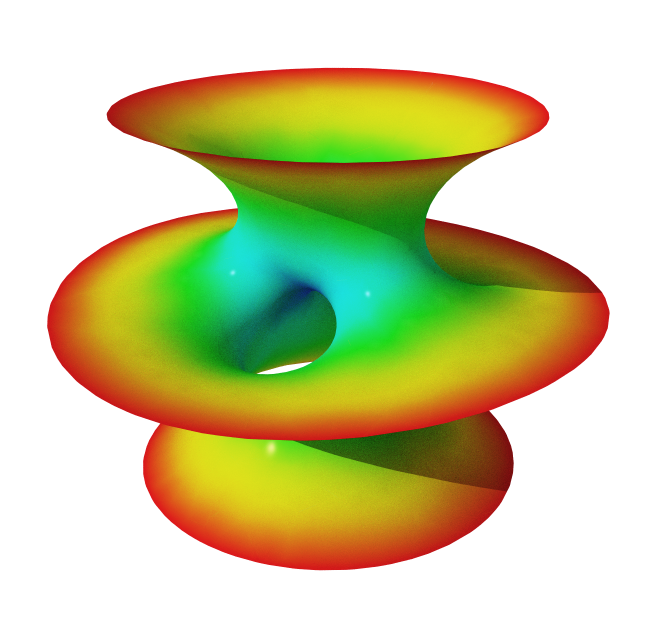
\includegraphics[width=\textwidth]{images/Costa's_Minimal_Surface.png}
            % \end{textblock*}

        \end{frame}
        
        \begin{frame}{Geodesics}
            \emph{Geodesics} $\gamma$ have a few equivalent interpretations.
            \begin{itemize}
                \item $\gamma$ is the shortest path between two points on $M$.
                \item $\gamma$ is the least curved path between two points on $M$.
                \item $\gamma$ is a trajectory of a free particle on $M$.
                \item $\gamma$ minimizes the Dirichlet energy.
            \end{itemize}
        \end{frame}
        
            \begin{frame}{Geodesics}
            \emph{Geodesics} $\gamma$ have a few equivalent interpretations.
            \begin{itemize}
                \item $\gamma$ is the shortest path between two points on $M$.
                \item $\gamma$ is the least curved path between two points on $M$.
                \item $\gamma$ is a trajectory of a free particle on $M$.
                \item \colorbox<1>{yellow}{$\gamma$ minimizes the Dirichlet energy.}
            \end{itemize}
        \end{frame}
        
        \begin{frame}{Minimal Surfaces}
             Fix a closed curve $\Gamma$ and a surface $\Sigma$ with $\partial \Sigma = \Gamma$. The following are equivalent definitions of a \emph{minimal surface}.
            \begin{itemize}
                \item $\Sigma$ minimizes the area functional.
                \item $\Sigma$ has zero mean curvature.
                \item $\Sigma$ is a critical point of the mean curvature flow.
                \item $\Sigma$ minimizes the Dirichlet energy.
            \end{itemize}
        \end{frame}
        
        \begin{frame}{Minimal Surfaces}
             Fix a closed curve $\Gamma$ on $M$ and a surface $\Sigma$ with $\partial \Sigma = \Gamma$. The following are equivalent definitions of a \emph{minimal surface}.
            \begin{itemize}
                \item $\Sigma$ minimizes the area functional.
                \item $\Sigma$ has zero mean curvature.
                \item $\Sigma$ is a critical point of the mean curvature flow.
                \item \colorbox<1>{yellow}{$\Sigma$ minimizes the Dirichlet energy.}
            \end{itemize}
        \end{frame}
    
        
    \subsection{Framework}
    
    \begin{frame}{The Working Example}
    \begin{itemize}
        \item Consider an $n$-dimensional membrane $N$ that undergoes stretching. 
        \item This stretching costs energy and is unfavorable. 
        \item We wish to find the membrane $N$ that minimizes this energy cost.
    \end{itemize}
    \end{frame}
    
    \begin{frame}{One Dimension}
        \begin{figure}
            \centering
            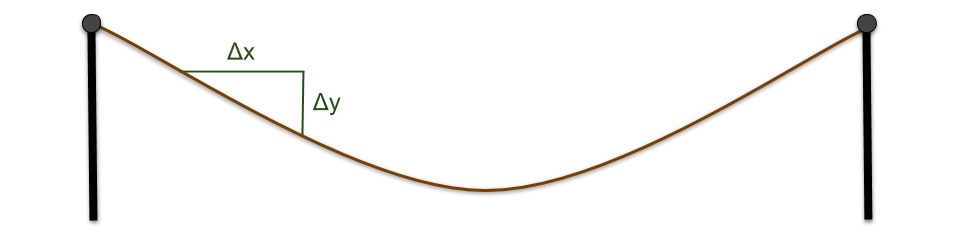
\includegraphics[width=.95\textwidth]{images/Dirichlet_Energy.png}
        \end{figure}
        For a 1-dimensional membrane given by $y=u(x)$ the increase in length from stretching is approximately
        \begin{align*}
            \sqrt{(\Delta x)^2+(\Delta y)^2}-\Delta x &= \left(\sqrt{1 + \left( \frac{\Delta y}{\Delta x}\right)^2} - 1\right)\Delta x\\
            \implies&= \frac{1}{2}\left\|\frac{du}{dx}\right\|^2dx
        \end{align*}
    \end{frame}


\begin{frame}{The Dirichlet Energy}
\begin{definition}
    The \emph{Dirichlet energy} measures stretching of the whole $n$-dimensional membrane. It is defined as the functional
    \[
    \mathcal{E}\colon H^1(\Omega) \to \R
    \]
    defined by
    \[
    \mathcal{E}[u]= \int_\Omega \frac{1}{2} \|\nabla u\|^2 = \int_\Omega \frac{1}{2} \langle \nabla u, \nabla u \rangle 
    \]
\end{definition}
\end{frame}
    
        % A bit unnecessary
        % \begin{frame}{Gradient Fields}
        % Given a scalar field $f(x_1,\dots,x_n)$, we can take $\nabla f$ as a vector field that points in the direction of steepest ascent.
        % \begin{figure}[H]
        %     \centering
        %     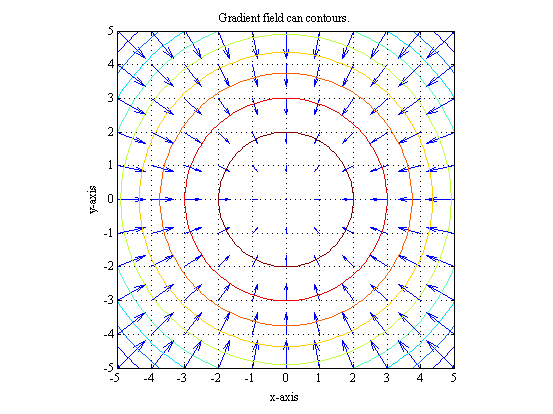
\includegraphics[width=.5\textwidth]{images/gradient_level_curves.png}
        %     \caption{Relationship between the level curves and gradient of a scalar field $f(x,y)$.}
        %     \label{fig:gradient_level_curves}
        % \end{figure}
        % \end{frame}
    
        
        

        
      
        
    
\section{PDEs and Geometry}

\subsection{Harmonic Maps}

\begin{frame}{Harmonic Maps}
    \begin{definition}
    A \emph{harmonic map} is a map that stationary point the Dirichlet energy functional
    \end{definition}
    
    \begin{remark}
    We can extend the Dirichlet energy to maps between Riemannian manifolds.
    \end{remark}
\end{frame}

\begin{frame}{Stationary Points}
    \begin{question}
        What is a stationary point of a functional?
    \end{question}
    \pause
    \begin{answer}
        It is an analogous definition to stationary points for functions.
    \end{answer}
\end{frame}

\begin{frame}{Stationary Points of Functions}
\begin{definition}
    Consider a function $f\colon \Omega \to \R$, then a \emph{stationary point} $(p_1,\dots,p_n)\in \Omega$ satisfies
    \[
    \nabla_{\mathbf{e}_i} f(p_1,\dots,p_n) = 0 \quad \forall \mathbf{e}_i \in \{\mathbf{e}_1,\dots,\mathbf{e}_n\},
    \]
    where $\nabla_{\mathbf{e}_i}$ is the directional derivative in direction $\mathbf{e}_i$.
    \end{definition}
\end{frame}

\begin{frame}{Stationary Points of Functionals}
\begin{definition}
    Consider a functional $\mathcal{E}\colon H^1(\Omega) \to \R$, then a \emph{stationary point} $u\in H^1(\Omega)$ satisfies
    \[
    \delta_v \mathcal{E}[u]=0\quad \forall v \in H^1_0(\Omega),
    \]
    where $\delta_v$ is a variation in ``direction" $v$.
    \end{definition}
\end{frame}

\begin{frame}{The Laplace Equation Example}
        Consider a variation in direction $v$ of the Dirichlet energy functional
        \begin{align*}
        \delta_v \mathcal{E}[u] \coloneqq \left.\frac{d}{d\epsilon} \mathcal{E}[u+\epsilon v]\right|_{\epsilon=0}&=0 \\
        \int_\Omega \nabla u \cdot \nabla v&= 0,
        \end{align*}
        which is the weak form of the Laplace equation,
        \[
        -\Delta u = 0.
        \]
        \begin{remark}
        $\implies$ Solutions to the Laplace equation are harmonic maps.
        \end{remark}
        \end{frame}
        
    \subsection{Gradient Flow}
     
        \begin{frame}{Finding Harmonic Maps}
            \begin{question}
                Is there any easier way to find harmonic maps?
            \end{question}
            \pause
            \begin{answer}
                Yes.  We can flow to the stationary points of functionals via the gradient flow.
            \end{answer}
        \end{frame}
        
\begin{frame}{Gradient Flow}
        In finite dimensions, (negative) gradient flow is given by following the path of steepest descent that limits to a stationary point.
        \begin{figure}[H]
            \centering
            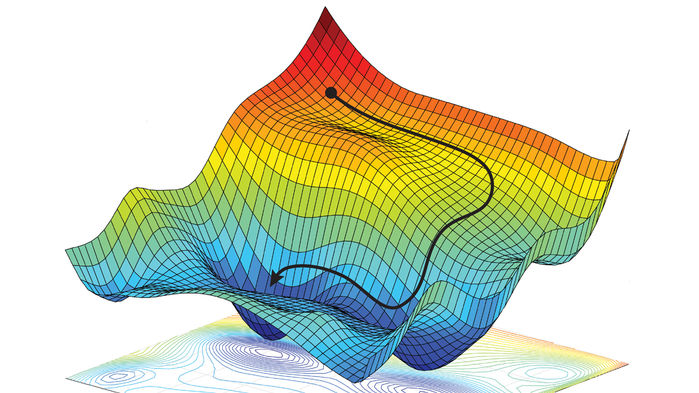
\includegraphics[width=.6\textwidth]{images/gradient_descent_surface.jpg}
            \caption{Thinking of our function as a surface, we let our curve follow the gradient field over time.}
            \label{fig:gradient_flow_surface}
        \end{figure}
        \end{frame}
        
        
    
        % May not be necessary really        
        % \begin{frame}{A Few Questions}
        %     \begin{itemize}
        %         \item How do we know we will find a (local) minimizer?
        %         \item When is this local minimizer global?
        %         \item 
        %     \end{itemize}
        % \end{frame}
        
 
        
        \begin{frame}{Finite Dimensional Gradient Flow}
        
        \begin{definition}
        The \emph{gradient flow} is a curve $\boldsymbol{\gamma}$ such that
        \[
        \frac{\partial \boldsymbol\gamma}{\partial t} = -\nabla f.
        \]
        Equivalently, the gradient flow in direction $\mathbf{e}_i$ is given by
            \[
            \langle \mathbf{e}_i ,\boldsymbol{\dot{\gamma}}\rangle = -\nabla_{\mathbf{e}_i} f \quad \forall \mathbf{e}_i \in \{\mathbf{e}_1,\dots,\mathbf{e}_n\}.
            \]
        \end{definition}
        \end{frame}
        
        \begin{frame}{Computational Method}
            This is feasible to compute given any starting position by
            \begin{figure}[H]
                \centering
                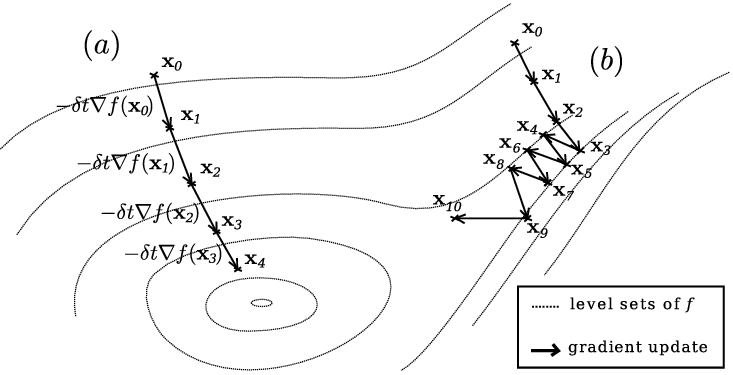
\includegraphics[width=.6\textwidth]{images/gradient-trajectory.png}
                \caption{A computational trajectory of the gradient flow.}
                \label{fig:gradient_trajectory}
            \end{figure}
        \end{frame}
        
        
  
        
    
        \begin{frame}{Gradient Flow in $H^1$}
        \begin{definition}
            The \emph{gradient flow} in $H^1(\Omega)$ in direction $v$ is
            \[
            \left\langle v,\frac{\partial u}{\partial t}\right\rangle=-\delta_v \mathcal{E}[u]
            \]
            and will give us a weak form of a PDE.
        \end{definition}
        \end{frame}
        
        \begin{frame}{The Heat Equation Example}
            We can then take the gradient flow in direction $v$ by
            \begin{align*}
            \left\langle v,\frac{\partial u}{\partial t}\right\rangle&=-\delta_v \mathcal{E}[u]\\
            &\downarrow\\
            \int_\Omega v\frac{\partial u}{\partial t} &= -\int_\Omega \nabla u \cdot \nabla v 
            \end{align*}
            Which is the weak form of the source free Heat equation
            \[
            \frac{\partial u}{\partial t} - \Delta u = 0.
            \]
        \end{frame}
        
        
    \begin{frame}{Answering the Question}
        \begin{question}
        What is a stationary point for the functional $\mathcal{E}$?
        \end{question}
        
        \pause
        \begin{answer}
        The limit as $t\to \infty$ of our gradient flow.
        \end{answer}
    \end{frame}
    
    \begin{frame}{Computational Method}
    \begin{itemize}
        \item The process for computing the gradient flow is similar to that in $\R^n$.
        \item Here and we use a finite element basis and compute the directional variation along this basis.
    \end{itemize}
         
    \end{frame}
    
    %Maybe not necessary really
    % \begin{frame}{Explicit Example with Fourier Basis}
    %     Fix $\Omega = (0,1)$ and consider $H^1_0(\Omega)$.
    %     \begin{enumerate}[1.]
    %         \item We can choose an initial condition, $u(x,0)=u_0(x)$.
    %         \item An approximate finite basis is $\sin(n\pi x)$ for $n=1,2,\dots N$.
    %         \item Project $u_0(x)$ onto this basis.
    %         \item Step forward in time to get $u_1(x)$ and project onto this basis.
    %         \item Continue and let $t\to \infty$ and we find that $u_\infty(x)$ is a solution to Laplace's equation.
    %     \end{enumerate}
        
    % \end{frame}
    
    \subsection{Geometry and Other Applications}
    
    \begin{frame}{Geodesics in $\R^n$}
        Take a curve $\boldsymbol{\gamma}\colon [0,1]\to \R^n$.  Then the Dirichlet energy is
        \[
        \mathcal{E}[\boldsymbol{\gamma}] = \int_{[0,1]} \frac{1}{2}\|\boldsymbol{\dot{\gamma}}\|^2 = \int_{[0,1]}\frac{1}{2} \langle \velocity, \velocity \rangle.
        \]
        Note that the quantity
        \[
        \frac{1}{2}\langle \velocity,\velocity \rangle
        \]
        is the kinetic energy of a free particle.
    \end{frame}
    
    \begin{frame}{Geodesics in $\R^n$}
        \begin{enumerate}[1.]
            \item Fix the endpoints to $\position(s)$, $\position(0)=p$ and $\position(1)=q$. 
            \item Define 
            \[
            \mathbf{u} \colon [0,1]\times [0,\infty) \to \R^n
            \]
            with
            \[
            \mathbf{u}(s,0)=\position(s),\quad \mathbf{u}(0,t)=p,\quad \mathbf{u}(1,t)=q.
            \]
            \item Define $\mathbf{v}(s,t)$ and force
            \[
            \mathbf{v}(0,t)=\mathbf{0},\quad \mathbf{v}(1,t)=\mathbf{0}.
            \]
        \end{enumerate}
    \end{frame}
    
    \begin{frame}{Geodesics in $\R^n$}
        \begin{enumerate}[4.]
            \item Then the gradient flow is
            \begin{align*}
            \int_{[0,1]} \mathbf{v}\cdot  \frac{\partial \mathbf{u}}{\partial t} ds&= - \delta_\mathbf{v} \mathcal{E}[\mathbf{u}]\\
            &= -\int_{[0,1]} \frac{\partial \mathbf{u}}{\partial s}\cdot \frac{\partial \mathbf{v}}{\partial s}ds\\
            &= \int_{[0,1]} \frac{\partial^2 \mathbf{u}}{\partial s^2}\cdot \mathbf{v} ds - \underbrace{\int_{\{0,1\}} \frac{\partial \mathbf{u}}{\partial s}\cdot \mathbf{v}ds}_{\textrm{equals 0}}.
            \end{align*}
        \end{enumerate}
    \end{frame}
    
    \begin{frame}{Geodesics in $\R^n$}
        \begin{itemize}
            \item[5.] With sufficient smoothness we get
            \[
            \frac{\partial \mathbf{u}}{\partial t} -\frac{\partial^2 \mathbf{u}}{\partial s^2}=\mathbf{0}.
            \]
            \item[6.] If we take the limit $t\to \infty$, then
            \[
            -\frac{\partial^2 \mathbf{u}}{\partial s^2}=\mathbf{0}.
            \]
            \item[7.] So we have the components
            \[
            u_i = a_i s + b_i
            \]
            and $\mathbf{u}$ is a straight line.
        \end{itemize}
    \end{frame}
    
    \begin{frame}{Geodesics on $M$}
        On a smooth Riemannian manifold $M$, the Dirichlet energy for a curve $\position \colon [0,1] \to M$ is
        \[
        \mathcal{E}[\position] = \int_{[0,1]} \frac{1}{2} \langle \velocity,\velocity \rangle_{g} = \int_{[0,1]} \frac{1}{2}  g_{ij} \dot{\gamma}^i \dot{\gamma}^j dt,
        \]
        where $\langle \cdot,\cdot \rangle_g$ is the position dependent inner product (Riemannian metric).\\
        \vspace*{.5cm}
        \noindent \textbf{Advantage:} Can handle constraints such as curves confined to a sphere.
    \end{frame}
    

    
    \begin{frame}{Minimal Surfaces in $\R^3$}
    \begin{enumerate}[1.]
        \item Fix a closed curve $\Gamma \colon S^1 \to \R^3$.
        \item Let $\Sigma$ be a surface defined by a function $\mathbf{u}\colon D \times [0,\infty) \to \R^3$.
        \item We require $\textrm{Graph}(\mathbf{u}|_{\partial D}(\mathbf{x},t))=\Gamma$.
        \item Then do the gradient flow with the Dirichlet energy
        \[
        \int_{D} v \frac{\partial u}{\partial t} d\mathbf{x} = \int_{D} \nabla v\cdot {\nabla u} d\mathbf{x}
        \]
    \end{enumerate}
    \end{frame}
    
    \begin{frame}{On a Manifold}
        The Dirichlet energy for a map $u \colon M \to N$ ($M$ compact) is
        \begin{align*}
        \mathcal{E}[u] &=\frac{1}{2} \int_{M} \|du\|^2 d\textrm{Vol}_M = \frac{1}{2} \int_{M}g^{ij}h_{\alpha \beta} \frac{\partial u^\alpha}{\partial x^i}\frac{\partial u^\beta}{\partial x^j}d\textrm{Vol}_M.
        \end{align*}
        A stationary point of this energy is a \emph{weakly harmonic map}.
        \begin{itemize}
            \item The matrix $\frac{\partial u^\alpha}{\partial x^i}$ is the Jacobian of the transformation.
            \item The Jacobian describes the stretching of space.
            \item Geodesics, minimal surfaces, and minimal submanifolds are harmonic.
        \end{itemize}
    \end{frame}
    
    
    \begin{frame}{From $\Omega$ to $\R^n$}
        Let $\mathbf{u}\colon \Omega \to \R^n$ so we can realize $\mathbf{u}$ as a vector field on $\Omega$. Then $g^{ij}=\delta^{ij}$ and $h_{\alpha \beta}=\delta_{\alpha \beta}$. We then get
        \[
        \mathcal{E}[u] = \frac{1}{2} \int_{\Omega} \|\textrm{Jac}(\mathbf{u})\|_{F}^2 d\mathbf{x}.
        \]
        with the Frobenius norm
        \[
        \|A\|_F = \sqrt{\sum_{i=1}^n \sum_{j=1}^n |a_{ij}|^2}.
        \]
    \end{frame}
    
% \begin{frame}{Constraints}
%         \begin{question}
%         Can every constrained optimization problem be placed as an optimization problem on a manifold (possibly with boundary)?
%         \end{question}
%     \end{frame}


\begin{frame}{Things to add/change}
\begin{itemize}
    \item Non-unique minimal surfaces with tennis ball
    \item Analogies with stretchable membranes. Especially when talking about minimal submanifolds.  Like stretching over a sphere and stuff. 
    \item Geodesics as rubber bands.
    \item The flow to a geodesic as pulling a rope tight.
    \item Organize the motivation/conclusion type stuff more
    \item Maybe just define the notion of a harmonic map
    \item 
    \url{https://en.wikipedia.org/wiki/Harmonic_map}
        
        uhh... should the $\phi^{-1}$ be a pullback instead of a preimage?
\end{itemize}
\end{frame}

      \begin{frame}{The Benefit of the Results}
            What's the point of what we'll do here?
            \begin{itemize}
                \item Provide a method to search for optimizers from arbitrary initial conditions.
                \item Create a framework to prove theorems such as existence and uniqueness.
            \end{itemize}
        \end{frame}
    
        
\end{document}